\documentclass[11pt]{article}
%\usepackage{fullpage,url}
\usepackage{url}
\usepackage{amsmath}
\usepackage{graphicx}
\usepackage{caption}
\usepackage{subcaption}

\usepackage[letterpaper,top=1in,bottom=1in,left=1in,right=1in,nohead]{geometry}

\setlength{\parindent}{0in}
\setlength{\parskip}{6pt}
\bibliographystyle{plain}

\DeclareMathOperator{\E}{E}
\DeclareMathOperator{\Var}{Var}
\DeclareMathOperator{\Unif}{Unif}
\DeclareMathOperator{\shrink}{shrink}

\begin{document}
\thispagestyle{empty}
{\large{\bf CS7640: Advanced Image Processing \hfill Danny Perry}}\\

{\LARGE{\bf Segmentation using Normalized Cuts}}
\vspace{0.2\baselineskip}
\hrule

\section{Introduction}
Segmentation is one of the ongoing, fundamental problems in image processing and computer vision. 
There are essentially three ways to think about segmentation: classification of pixels, the delineation of boundaries, and partitioning the image into regions.
While a useful model to view the process, they three different methods are all related, and can be reformulated into each other.
Here I will be describing segmentation in the last form - that of partitioning the image into regions.

One interesting approach to segmentation is to model the image as a graph and make use of the extensive work in graph theory to solve the segmentation problem.
One idea in this area is to use a minimum graph cut to segment an image into regions, motivated by the goal of segmenting so that the affinity of the different regions is minimized.
\ref{shi2004} is a popular and interesting approach to this, because instead of using the standard cut, they normalize the cut using the association of each subgraph with the rest of the graph.
Normalizing the cut pushes the solution to reject segmentations that only minimize the number of connections between the two subgraphs and focus more on the cut weights.
The method is straightforward and will be the subject of this report.

\section{Graph Construction}

In any of the methods making use of graph theory, a graph needs to be generated making use of the image information.
For the normalized graph cut method \ref{shi2004} provide a general framework and then suggest a few specific mehtods of constructing the connections and their weights.

\section{Solution using Eigenanalysis}

\begin{figure}
\centering
\graphicspath{{images/}}
\begin{subfigure}[b]{0.4\textwidth}
\centering
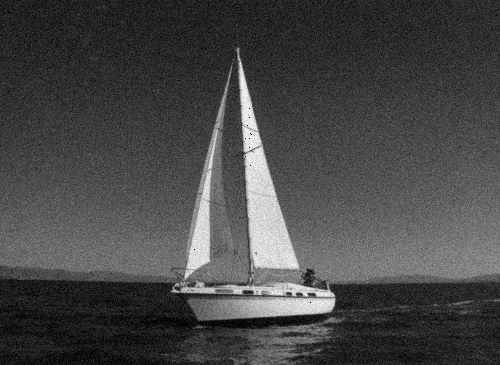
\includegraphics[width=\textwidth]{sailboat_10}
\caption{Noisy}
\label{sail:noise}
\end{subfigure}
\begin{subfigure}[b]{0.4\textwidth}
\centering
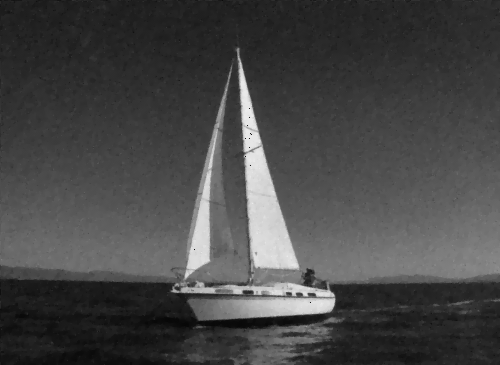
\includegraphics[width=\textwidth]{sailboat_10_ch}
\caption{Chambolle's}
\label{sail:ch}
\end{subfigure}
\begin{subfigure}[b]{0.4\textwidth}
\centering
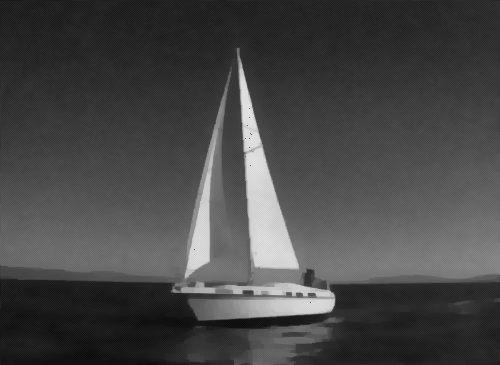
\includegraphics[width=\textwidth]{sailboat_10_pd}
\caption{Primal-Dual}
\label{sail:pd}
\end{subfigure}
\begin{subfigure}[b]{0.4\textwidth}
\centering
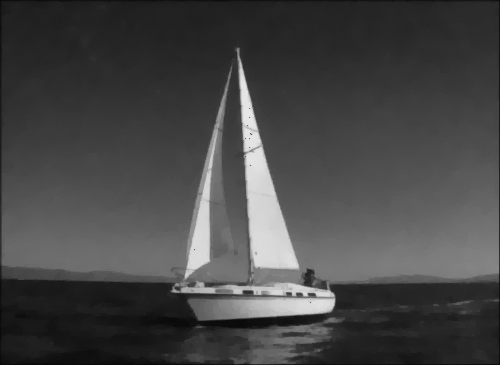
\includegraphics[width=\textwidth]{sailboat_10_sb}
\caption{Split-Bregman}
\label{sail:sb}
\end{subfigure}
\caption{Results of each algorithm on a noisy image of a sailboat.}
\label{fig:sailboat:dn}
\end{figure}

\begin{figure}
\centering
\graphicspath{{images/}}
\begin{subfigure}[b]{0.4\textwidth}
\centering
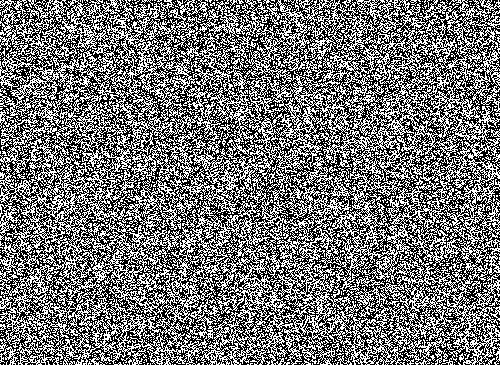
\includegraphics[width=\textwidth]{sail_gauss_diff}
\caption{Gaussian blur}
\label{sail:gauss:diff}
\end{subfigure}
\begin{subfigure}[b]{0.4\textwidth}
\centering
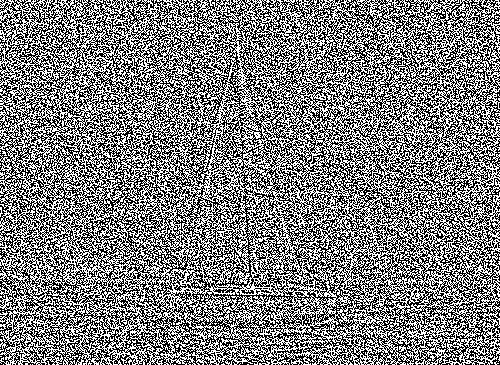
\includegraphics[width=\textwidth]{sail_ch_diff}
\caption{Chambolle's}
\label{sail:ch:diff}
\end{subfigure}
\begin{subfigure}[b]{0.4\textwidth}
\centering
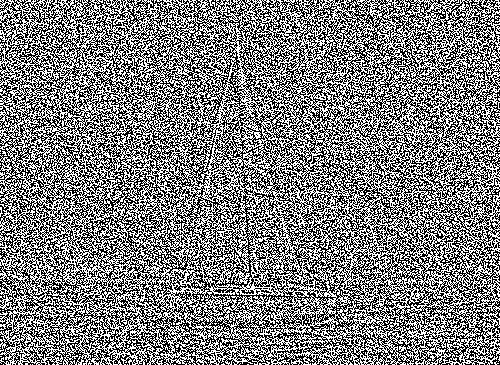
\includegraphics[width=\textwidth]{sail_pd_diff}
\caption{Primal-Dual}
\label{sail:pd:diff}
\end{subfigure}
\begin{subfigure}[b]{0.4\textwidth}
\centering
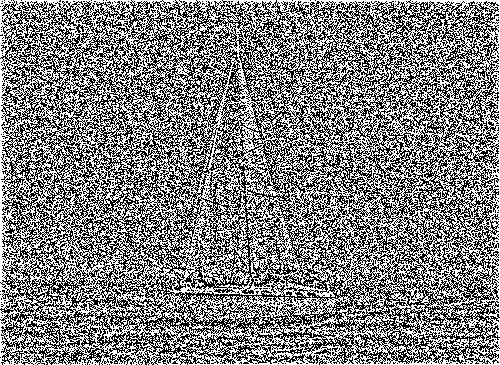
\includegraphics[width=\textwidth]{sail_sb_diff}
\caption{Split-Bregman}
\label{sail:sb:diff}
\end{subfigure}
\caption{Diff of each result with the noisy image, (a) shows the result of a standard Gaussian blur denoising using a width of 4.}
\label{fig:sailboat:diff}
\end{figure}




\bibliography{normalized_cuts}

\end{document}
